\chapter{Návrh aplikace}
    Návrh aplikace je velice důležitou fází projektu, ve které by mělo dojít ke sjednocení požadavků zadavatelů a reálného provedení. Vytvořením dobrého návrhu se zamezí případným kolizím a zároveň proběhne první interakce mezi zákazníkem a dodavatelem. Ze strany UČL byl vznesen požadavek, aby v aplikaci byl použit Bootstrap\footnote{domovská stránka: \url{https://v4-alpha.getbootstrap.com/}}, protože jsou na něj zvyklí. Databázové schéma bylo čistě na mém rozhodnutí.
    
    \section{Wireframy}

        Jedním z nejdůležitějších úkolů bylo navrhnout, jak budou jednotlivé stránky vypadat a kolik jich aplikace bude obsahovat. Základní rozložení stránek bylo na mém rozhodnutí. Design měl být jednoduchý, uživatelsky přívětivý a moderní. Tyto návrhy musely být a byly schváleny pracovníky UČL AV.
        
        Grafika měla být jednoduchá, bez složitých a obsáhlých prvků. Pro snadnější stylování aplikace byl použit Bootstrap. Jedná se o volně dostupnou knihovnu, která dovoluje stylovat vzhled aplikace pouze přídáním určitých tříd k elementům v HTML. Při dodržování pravidel Bootstrapu není potřeba vkládat obsáhlé CSS styly. Pomocí Bootstrapu lze poměrně snadno vytvořit responzivní aplikaci.
        
        Pro návrh GUI jsem se rozhodl použít webovou aplikaci Moqups\footnote{domovská stránka: \url{https://moqups.com/}}. Její bezplatná verze nabízí velké množství šablon pro grafické návrhy. Od základních prvků jako je tlačítko nebo nadpis, po mírně složitější formuláře. Velikou výhodou je, že Moqups má v nabídce prvky Bootstrapu. 
        
        \subsection{Login}
            Pro úvodní přihlašovací stránku jsem vybral jednoduchý formulář, ve kterém je email a heslo, viz obrázek \ref{fig:login}. Pozadí, které by se dalo v budoucím rozšíření měnit, je jako na všech ostatních stránkách bílé.
            
        \subsection{Hlavní stránka}
            Po úspěšném přihlášení do aplikace se zobrazí hlavní stránka, která je rozdělena do tří částí, jak je vidět na obrázku \ref{fig:main}. V hlavičce se nachází společně s nadpisem odkaz na seznam autorů a vydavatelů děl a vysouvací menu s možnostmi uživatele. Dále je zde filtr aplikovatelný na seznam zobrazených děl. Požadavek od UČL AV byla možnost filtrovat elektronickou literaturu podle autora, roku vydání, textu obsaženého v díle a statusu. Třetí část obsahuje samotný seznam děl. Tento seznam je ve tvaru tabulky se sloupci (\textit{název díla, autor, rok vydání, status}), odkaz na přílohy a nezbytné akce a tabulka se dá seřadit podle vybraných sloupců. U seznamu děl lze nastavit počet zobrazených děl a obsahuje rychlý vyhledávač v textu zobrazeným v tabulce.

        \subsection{Metadata}
            Na obrázku \ref{fig:metadata} je vidět rozložení stránky pro úpravu základních údajů o dílu. Opět se skládá ze tří částí. První obsahuje navigaci, dropdown pro přihlášeného uživatele a nadpis. Druhá část je věnována autorům a vydavatelům. V tomto oddílu bude umožněno přidávat a odebírat autora nebo vydavatele. Poslední sekce obsahuje formulář pro úpravu metadat literárního díla. Společně s pracovníky UČL AV byly vybrány atributy, které přímo nesouvisí s obsahem díla, nýbrž popisují samotnou publikaci. 
        
        \subsection{Přílohy}
            Součástí zadání práce je správa příloh, zejména scanů stránek. Přílohám se věnuje právě tento segment. Obsahem wireframu \ref{fig:attachments} jsou naskenované jednotlivé stránky daného literárního díla. V horní části se opět objevuje navigace, uživatelské funkce a nadpis. Následuje sekce věnovaná hromadnému uploadu skenů do níže zobrazené fotogalerie.
            
        \subsection{Autoři a vydavatelé}
            Pro správu autorů a vydavatelů byl použit návrh zobrazený v příloze \ref{fig:authPub}. V horní části se vyskytuje navigace, nezbytné funkce a nadpis. Dále je zde umístěna tabulka záznamů, ve kterých lze snadno vyhledávat. Každý záznam lze upravit a smazat. Pro upravení záznamu byl navržen wireframe z obrázku \ref{fig:edit}, který obsahuje navigaci, funkce pro uživatele a zjednodušený formulář. Formuláře pro upravení vydavatele nebo autora jsou totožné.
            
            \begin {figure}[H]\centering
                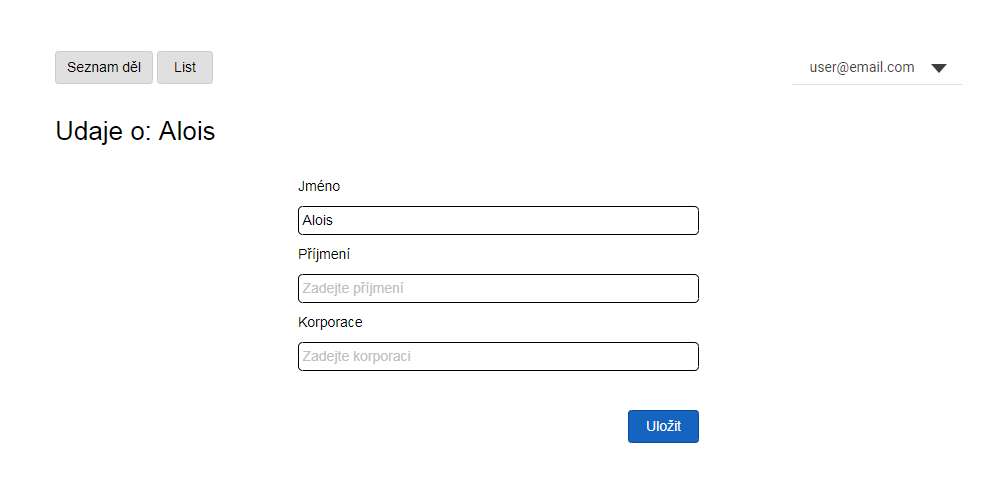
\includegraphics[width=\textwidth]{images/edit}
                \caption {Úprava autora}
                \label {fig:edit}
            \end{figure}
            
        \subsection{Text}
            Nejdůležitějším prvkem aplikace byla bezesporu možnost upravovat text literárního díla. Pro tuto funkci byla navržena stránka z obrázku \ref{fig:text}. Jako u předešlých wireframů, horní část se věnuje navigaci, funkcím uživatele a nadpisu. Dále je vidět rozložení stránky na dva oddíly. Jeden pro text knihy a druhý pro možnost vkládání značek. Menu vpravo bylo navrženo vzhledem k nadměrné velikosti první části tak, aby bylo viditelné, když se uživatel posune níž.
            
    \section{Databázové schéma}
        Neméně duležitou součástí projektu byla databáze. Ze strany UČL AV nebyly vzneseny žádné požadavky na podobu databáze, proto se mohlo schéma přizpůsobit dle potřeby aplikace.
        
        Pro model databáze byla použita webová aplikace\footnote{domovská stránka: \url{https://www.quickdatabasediagrams.com/}}. Schéma je navrženo minimalisticky, ale tak aby zároveň pokrývalo veškeré potřeby aplikace. Výsledný návrh databáze na obrázku \ref{fig:schema}, obsahuje 5 tabulek s jednoduchými vazbami.
        
        \begin {figure}[H]\centering
            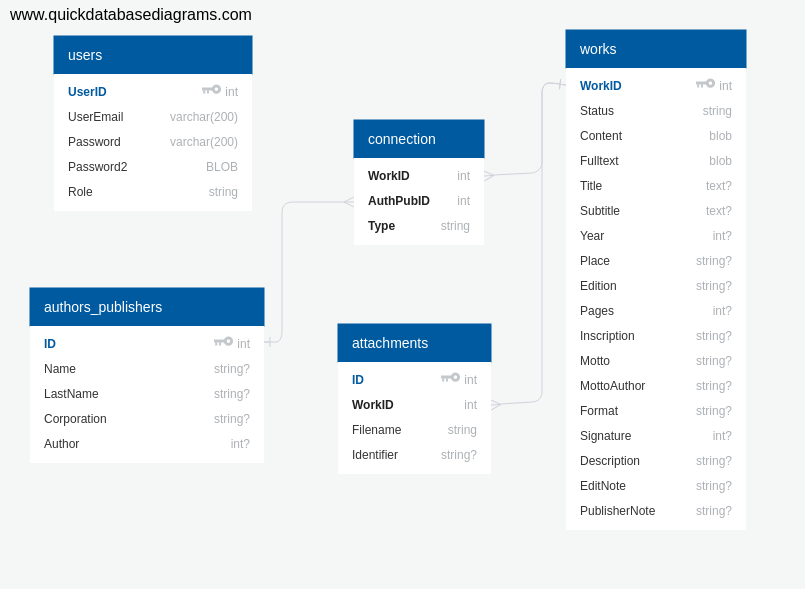
\includegraphics[width=\textwidth]{images/schema}
            \caption {Databázové schéma}
            \label {fig:schema}
        \end{figure}
        
        V tabulce uživatelů je uloženo (\textit{UserID}), (\textit{UserEmail}) a heslo rozdělené do dvou sloupečků viz sekce \ref{autentizace}. Uživatelské role jsou identifikovány pomocí sloupce Role.
        
        Duležitá tabulka je (\textit{author\_work}). Obsahuje reference na tabulky (\textit{works}) a (\textit{authors\_publishers}). Třetím atributem je typ spojení. Tento typ určuje, jestli je spojen autor nebo vydavatel díla. Každý záznam v tabulce propojuje dílo a autora nebo vydavatele. Primárním klíčem je celá trojice.
        
        (\textit{AuthPubID}), (\textit{Name}), (\textit{LastName}), (\textit{Corporation}) a (z\textit{Author}) jsou atributy tabulky (\textit{authors\_publishers}). Záznamem může být reálná osoba, její pseudonym nebo společnost. V případě pseudonymu odkazuje záznam na reálnou osobu. Tuto referenci obsahuje sloupec (\textit{Author}), ve kterém je (\textit{AuthPubID}) reálné osoby zaznamenané v (\textit{authors\_publishers}) nebo je prázdný.
        
        Nejobsáhlejší tabulka se nazývá (\textit{works}). Obsahuje všechny základní informace o dílu: název díla (\textit{Title}), podtitul (\textit{Subtitle}), datum publikace (\textit{Year}), místo vydání (\textit{Place}), pořadí vydání (\textit{Edition}), počet stran sbírky (\textit{Pages}), věnování autora (\textit{Inscription}), motto (\textit{Motto}), autor motta (\textit{MottoAuthor}), formát naskenovaného díla (\textit{Format}), podpis (\textit{Signature}), popis díla (\textit{Description}) a poznámka k vydání (\textit{EditNote}). Ve (\textit{works}) je atribut (\textit{Status}), který indikuje momentální stav díla. (\textit{Status}) může nabývat hodnot domluvených s UČL AV Nové, Rozpracováno, Zkontrolováno a Hotovo. Celý text včetně tagů je ve sloupci (\textit{Content}). Dále tabulka (\textit{works}) obsahuje sloupec (\textit{Fulltext}), ve kterém je text díla bez tagů.
        
        Poslední tabulka (\textit{attachments}) je pro přílohy přidružené k dílům. Obsahuje (\textit{AttachmentID}), referenci na dílo (\textit{WorkID}), (\textit{Filename}) a poznámku k obrázku (\textit{Identifier}).
        
    \section{Autentizace} \label{autentizace}
        Součástí zadání je požadavek na možnost autentizace. Ze strany ústavu nebyl vznesem žádný požadavek na ochranu hesel, proto jsem si způsob zabezpečení mohl vybrat. Heslo je zahashované pomocí sha256. Pro větší bezpečnost hesla jsem přidal metodou solení hesla\cite{salt} tzn., že se k uživatelskému heslu přidává náhodný text.
